\section{ Предобработка и анализ стационарности временного ряда }

\subsection{ Моделирование временного ряда }

Для анализа было смоделировано два временных ряда (ВР) с числом отсчётов $N = 500$ и длительностью $T = 1$с.

\begin{equation*}
	y_1 = a_0 \sin \left( a_1 \cdot 2\pi \cdot t\right) + a_2 \cdot e
\end{equation*}
\begin{equation*}
	y_3 = e^{0,1\cdot t} + 2 \cdot e,
\end{equation*}
\begin{equation*}
	\text{где } e \sim N(0, 1), \; a_0 = 0,4,\;a_1 = 0,015,\; a_2 = 0,63 
\end{equation*}

Генерация данных ВР приведена в листинге \ref{generation}. Полученные временные ряды представлены на рис. \ref{graphs}.

В структуре генерирующей формулы обоих временных рядов заложена неслучайная составляющая. Для $y_1(t)$ заложена периодическая составляющая, а для $y_3(t)$ заложен тренд, представляющий собой экспоненту. Визуально на графиках временных рядов сложно предположить о наличии этих составляющих.

\noindent{
\begin{center}
	\begin{minipage}{.48\textwidth}
		\centering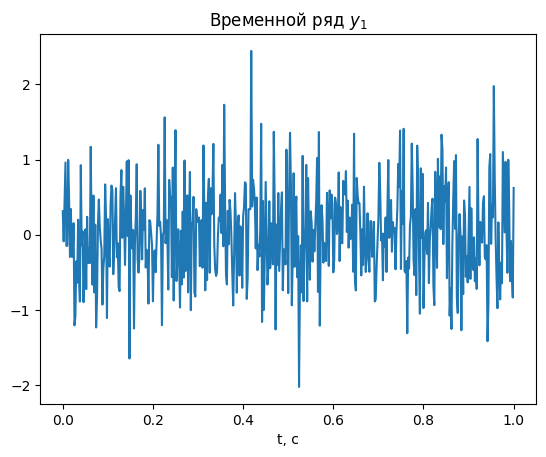
\includegraphics[width=\textwidth]{png/y1.png}
		а)
	\end{minipage}
	\begin{minipage}{.48\textwidth}
		\centering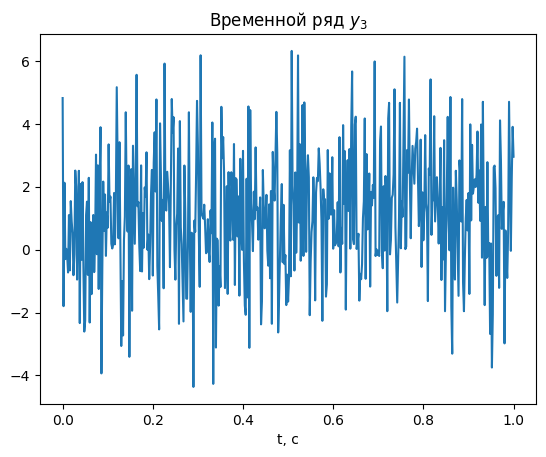
\includegraphics[width=\textwidth]{png/y3.png}
		б)
	\end{minipage}
	\captionof{figure}{Графики: а)\,$y_1 (t)$, б)\,$y_3 (t)$}
	\label{graphs}
\end{center}
}

\subsection{Обработка аномальных наблюдений}

Для обнаружения аномалий построим эллипс рассеяния набора данных $\left(x\;y\right)=\left( \Delta y\;\;\nabla y \right)$. Для этого рассмотрим ковариационную матрицу нормированных данных $C$.

\begin{equation*}
	\Sigma = \begin{bmatrix}
		\sigma_x ^ 2 & \sigma_{xy} \\ 
		\sigma_{xy} & \sigma_y ^ 2
	\end{bmatrix} \Rightarrow
	C = \left. \Sigma \right|_{\sigma_x = \sigma_y = 1} = \left.\begin{bmatrix}
		\sigma_x^2 & \rho_{xy} \sigma_x \sigma_y \\
		\rho_{xy} \sigma_x \sigma_y & \sigma_y^2
	\end{bmatrix} \right|_{\sigma_x = \sigma_y = 1} = \begin{bmatrix}
		1 & \rho_{xy} \\
		\rho_{xy} & 1
	\end{bmatrix}
\end{equation*}

Собственные значения такой матрицы будут равны:

\begin{equation}
	\lambda_{1,\,2} = 1 \pm \rho_{xy}
\end{equation}

Система собственных векторов в данном случае будет расположена под углом 45$^\circ$ относительно осей $Oxy$. Для облака рассеяния нормированных данных длины полуосей эллипса будут равны:

\begin{equation}
	l_{1,\,2} = \sqrt{\lambda_{1,\,2}}
\end{equation}

Для перехода от нормированных данных $(x_0\;y_0)$ к исходным $(x\;y)$ эллипс масштабируется c учётом стандартных отклонений при помощи растягивания $S$:
\begin{equation}
	\begin{bmatrix}
		x \\ y
	\end{bmatrix} = \underbrace{\begin{bmatrix}
		\sigma_x & 0 \\ 0 & \sigma_y
	\end{bmatrix}}_{S} \cdot \begin{bmatrix}
		x_0 \\ y_0
	\end{bmatrix}
\end{equation}


\begin{figure}
	\centering
	\includestandalone[width=0.66\textwidth]{ellipse_illustration}
	\caption{Масштабирование эллипса рассеяния для заданной доверительной вероятности}
	\label{ellipse_ill}
\end{figure}


Вспомним, что рассматривается набор данных $\left( \Delta y\;\;\nabla y \right)$. При сравнивании значений по модулю, все значения кроме $\Delta y_N$ и $\nabla y_1$ встречаются в обоих выборках $\Delta y,\;\nabla y$. Это значит, что дисперсии практически равны: $\sigma^2_x = \sigma^2_y$, и оператор растягивания $S$ сохранит угол 45$^\circ$ между базисом собственных векторов и исходной системы координат $Oxy$.

В написанной функции построения эллипса рассеяния (листинг \ref{conf_ellipse}) можно задавать значение доверительной вероятности, по умолчанию $p=0,99$. На вход функции подаётся вектор $(x\;y)$, и предполагается, что этот вектор имеет двумерное нормальное распределение. 

Для учёта доверительной вероятности эллипс рассеяния масштабируется в соответствии с множителем стандартного отклонения (рис. \ref{ellipse_ill}), показывающим сколько стандартных отклонений должно быть охвачено:
\begin{equation*}
	n_\sigma = q_{\frac{1+p}{2}},
\end{equation*}
где $q_{\frac{1+p}{2}}$ -- квантиль для стандартного нормального распределения. Такое масштабирование сделает сам эллипс кривой, охватывающей $p$ вероятности двумерного нормального распределения.

В качестве входных данных при построении эллипса рассеяния используются передние и задние конечные разности. По оси $X$ имеем $\Delta y = y[k+1] - y[k]$, по оси $Y$: $\nabla y = y[k] - y[k-1]$. Все значения, которые оказываются вне эллипса рассеяния во II и IV квадрантах -- считаются аномальными. Аномальные значения заменяются средним значением между соседними отсчётами во временном ряду.

Полученные эллипсы рассеяния для $y_1(t)$, $y_3(t)$ представлены на рис. \ref{graph_ellipse}. Они были получены в результате программы, представленной в листинге \ref{plot_ellipse}. На графике оранжевым представлены наблюдения, которые были приняты аномальными и заменены средним значением.


\noindent{
	\begin{center}
		\begin{minipage}{.48\textwidth}
			\centering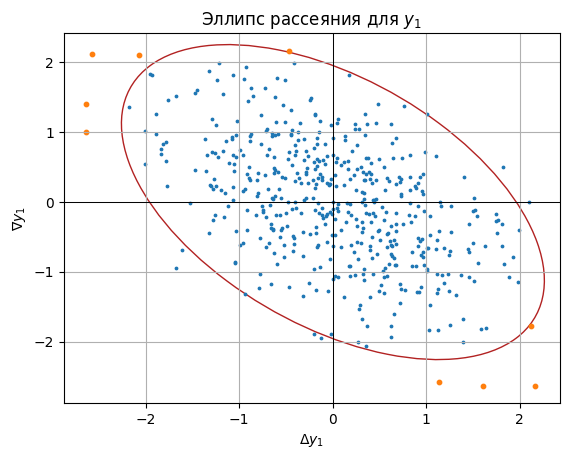
\includegraphics[width=\textwidth]{png/y1_ell.png}
			а)
		\end{minipage}
		\begin{minipage}{.48\textwidth}
			\centering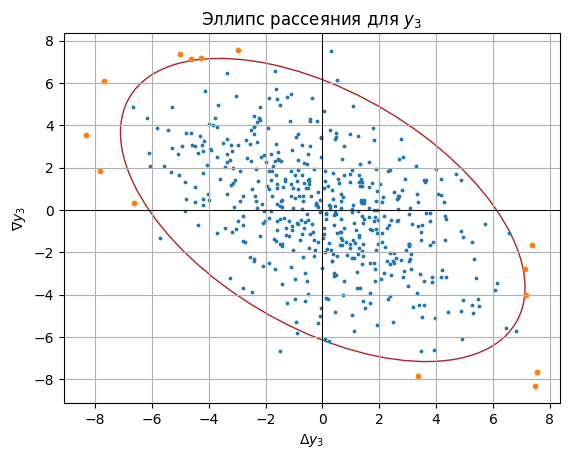
\includegraphics[width=\textwidth]{png/y3_ell.png}
			б)
		\end{minipage}
		\captionof{figure}{Эллипс рассеяния: а)\,$y_1 (t)$, б)\,$y_3 (t)$}
		\label{graph_ellipse}
	\end{center}
}

\subsection{Оценка стационарности}

Для оценки стационарности временных рядов они были разбиты на 10 блоков по 50 значений. В каждом блоке была рассчитана оценка математического ожидания и дисперсии (листинг \ref{stationary_prog}):
\begin{equation}
	\hat{m}_x = \frac{1}{N} \sum_{i=1}^N x_i
\end{equation}
\begin{equation}
	\hat{\sigma}_x^2 = \frac{1}{N-1} \sum_{i=1}^N (x_i - \hat{m}_x)^2 
\end{equation}

Полученные графики оценок представлены на рис. \ref{graph_blocks}. Визуально по ним сложно утверждать о том, что параметры как либо изменяются. Лишь для $y_3(t)$ можно предположить о слабом изменении математического ожидания. 

Критерий серий говорит о стационарности математического ожидания и дисперсии по результату анализа этих же графиков (листинг \ref{series_result}). 

Для обоих сигналов критерий Колмогорова-Смирнова для нормального распределения не выполняется. Это говорит о том, что сами сигналы нельзя считать просто нормально распределёнными.

Проанализируем автокорреляционные функции и спектральные плотности мощности для этих сигналов. Автокорреляционные функции представлены на рис. \ref{acorr_graphs}, а спектральные плотности мощности на рис. \ref{csd_graphs}.

{
	\captionof{lstlisting}{Вывод критерия серий}
	\vspace{-1.5em}
	\label{series_result}
	\begin{minted}[frame=lines,fontsize=\footnotesize,breaklines=true]{text}
По результату критерий серий "Тренд в m(y_1) отсутствует - True"
По результату критерий серий "Тренд в var(y_1) отсутствует - True"
По результату критерий серий "Тренд в m(y_3) отсутствует - True"
По результату критерий серий "Тренд в var(y_3) отсутствует - True"

Характеристики y1
Математическое ожидание - 0.024
Дисперсия - 0.383
Асимметрия - 0.179
Эксцесс - 0.254
Тест на нормальность Колмогорова-Смирнова - pvalue=9.5e-08

Характеристики y3
Математическое ожидание - 1.121
Дисперсия - 3.844
Асимметрия - 0.049
Эксцесс - -0.132
Тест на нормальность Колмогорова-Смирнова - pvalue=7.4e-64
	\end{minted}
}

\noindent{
	\begin{center}
		\begin{minipage}{.48\textwidth}
			\centering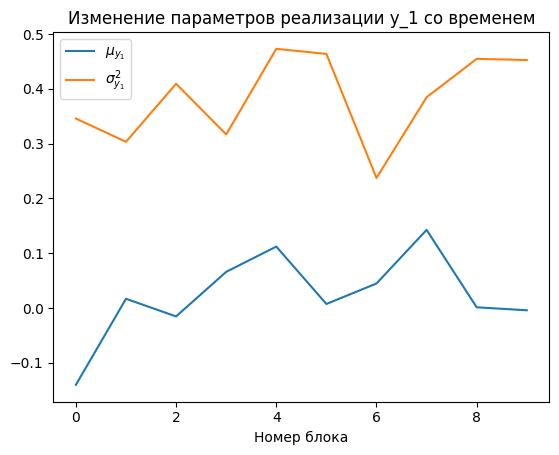
\includegraphics[width=\textwidth]{png/station_y1.png}
			а)
		\end{minipage}
		\begin{minipage}{.48\textwidth}
			\centering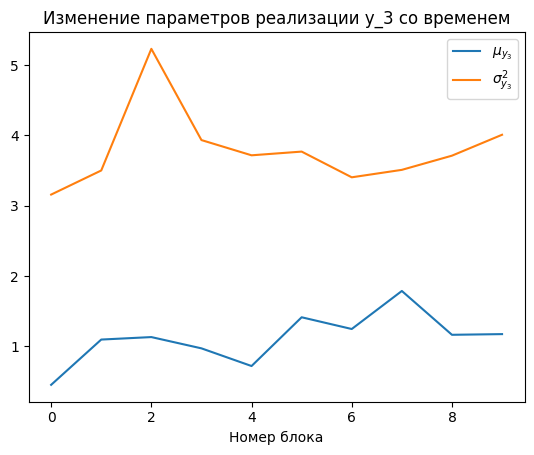
\includegraphics[width=\textwidth]{png/station_y3.png}
			б)
		\end{minipage}
		\captionof{figure}{Изменение параметров реализации: а)\,$y_1 (t)$, б)\,$y_3 (t)$}
		\label{graph_blocks}
	\end{center}
}

По автокорреляционным функциям можно сказать о наличии тренда в сигнале $y_3(t)$, т.к. эта функция явно не затухает до нуля, что говорит о наличии коррелированности между отсчётами временного ряда. Для $y_1(t)$ нельзя сказать о наличии тренда.

По графикам спектральной плотности мощности рассматриваемых сигналов нельзя сказать о наличии тренда или конкретной частоты. Мощность частот распределена довольно равномерно, что говорит о близости сигналов с белому шуму. В данном случае видно явное преобладание аддитивного шума, который был заложен в модель.

\noindent{
	\begin{center}
		\begin{minipage}{.48\textwidth}
			\centering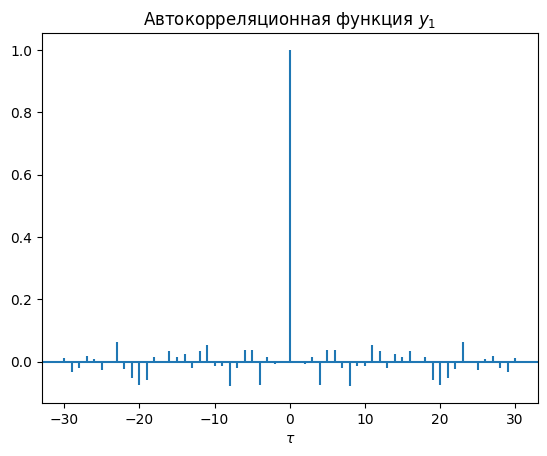
\includegraphics[width=\textwidth]{png/acorr_y1.png}
			а)
		\end{minipage}
		\begin{minipage}{.48\textwidth}
			\centering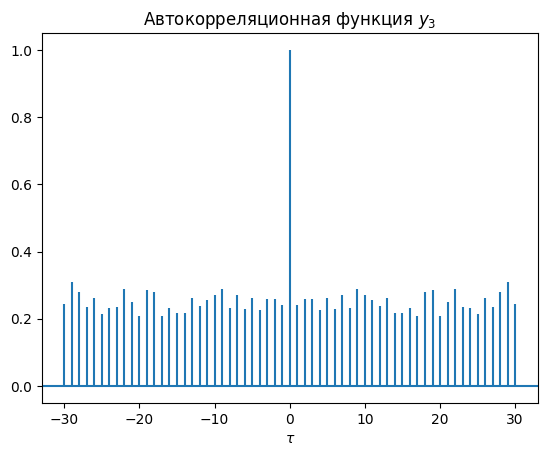
\includegraphics[width=\textwidth]{png/acorr_y3.png}
			б)
		\end{minipage}
		\captionof{figure}{Автокорреляционные функции: а)\,$y_1 (t)$, б)\,$y_3 (t)$}
		\label{acorr_graphs}
	\end{center}
}

\noindent{
	\begin{center}
		\begin{minipage}{.48\textwidth}
			\centering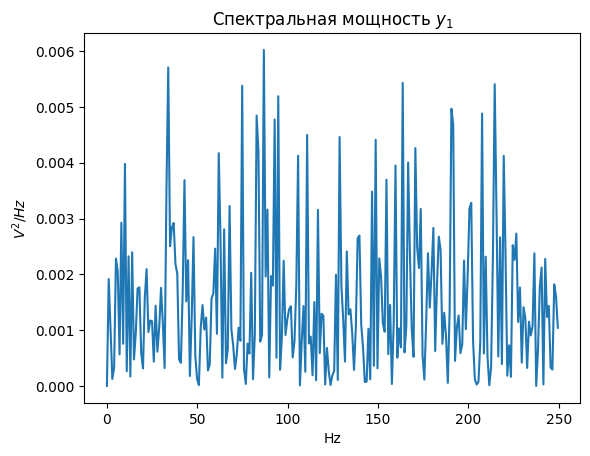
\includegraphics[width=\textwidth]{png/csd_y1.png}
			а)
		\end{minipage}
		\begin{minipage}{.48\textwidth}
			\centering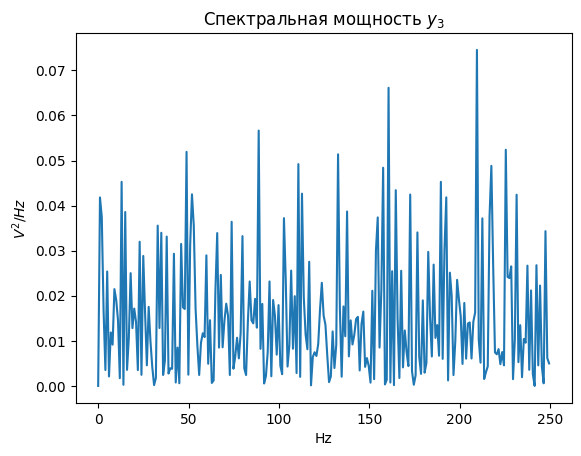
\includegraphics[width=\textwidth]{png/csd_y3.png}
			б)
		\end{minipage}
		\captionof{figure}{Спектральная плотность мощности: а)\,$y_1 (t)$, б)\,$y_3 (t)$}
		\label{csd_graphs}
	\end{center}
}
\section{Корреляционный и спектральный анализ ВР}

\subsection{Построение корреляционной функции}

Была написана функция \textit{correlation\_function}, которая строит корреляционную функцию (КФ) для двух данных сигналов. Реализация функции представлена в листинге \ref{corr_plot_prog}. Используется формула (\ref{Rxy}):
\begin{equation}
	\hat{R}_{xy}(k\Delta) = \frac{1}{N} \sum_{i=1}^{N-k} (x_i - \hat{m}_x)(y_{i+k} - \hat{m}_y)
	\label{Rxy}
\end{equation}

Полученные сигналы и корреляционные функции представлены на рис. \ref{corr_graph_1}-\ref{corr_graph_7}. Как видим, получили графики соответствующие теоретическим. Для белого шума автокорреляционная функция (АКФ) $R_{xx}(\tau) = \delta(\tau)$, для нескольких гармоник АКФ представляет собой сигнал тоже из нескольких гармоник, для сигнала с линейно-коррелированными отсчётами АКФ представляет собой затухающую экспоненту.

Таблица полученных интервалов максимальной корреляции $\tau_{\text{м.к.}}$ представлена на рис. \ref{max_corr_table}.

{
\foreach \i in {1,...,7}{
	\begin{center}
		\includegraphics[width=.8\linewidth]{png/corr_\i.png}
		\captionof{figure}{Корреляционная функция, пример \i}
		\label{corr_graph_\i}
	\end{center}
}
}

\begin{table}[h]
	\caption{Значение максимальных интервалов корреляции $\tau_{\text{м.к.}}$}
	\label{max_corr_table}
	\centering\begin{tabular}{|l|c|}
		\hline
		Тип сигнала                                        & $\tau_{\text{м.к.}}$ \\ \hline
		Постоянный                                         & 0                    \\ \hline
		Белый шум                                          & 1                    \\ \hline
		Несколько гармоник                                 & --                   \\ \hline
		Коррелированные отсчёты                            & 51                   \\ \hline
		Белый шум -- несколько гармоник                    & 0                    \\ \hline
		Несколько гармоник -- коррелированные отсчёты      & 0                    \\ \hline
		Коррелированные отсчёты -- коррелированные отсчёты & 0                    \\ \hline
	\end{tabular}
\end{table}

\subsection{Построение спектральной плотности мощности}

Были написаны функции \textit{periodogram} и \textit{estimate\_spe}, для построения периодограммы и применения к ней окон. Их реализация приведена в листинге \ref{csd_plot_prog}. Получили графики спектральных плотностей мощности, представленные на рис. \ref{csd_graph_1}-\ref{csd_graph_4}. Для всех окон параметр $M=100$. 

Можно отметить, что прямоугольное окно позволяет построить кусочно-непрерывную (в силу своей структуры) оценку спектральной плотности. Более гладкие дают остальные 3 окна.

Окно Бартлетта имеет излом в нуле, за счёт чего оценка получается кусочно-гладкой. Окно Хэмминга имеет разрыв 1-го рода, за счёт чего оценка тоже получается кусочно-гладкой. Самые гладкие оценки даёт окно Ханна, будучи аналитичной функцией.

За счёт разрыва 1-го рода на границе носителя окна Хэмминга пики на графике оказывают большее влияние на оценку СПМ в окрестности пика, чем окно Бартлетта и Ханна.

{
\foreach \i in {1,...,4}{
	\begin{center}
		\includegraphics[width=.8\linewidth]{png/csd_\i.png}
		\captionof{figure}{Спектральная плотность мощности, пример \i}
		\label{csd_graph_\i}
	\end{center}
}
}

Рассмотрим следующие сигналы:
\begin{equation*}
	x = 2\sin\left(102t \cdot 2\pi\right) + 1,7\sin\left(102,08t\cdot 2\pi\right) + 2,3\sin\left(110t\cdot 2\pi\right) + 0,2e
\end{equation*}
\begin{equation*}
	y = 1,6\sin\left(102,8t \cdot 2\pi\right) + 2,1\sin\left(110t\cdot 2\pi\right) + 2,0\sin\left(210t\cdot 2\pi\right) + 0,2e
\end{equation*}
\begin{equation*}
	\text{где } e \sim N(0, 1)
\end{equation*}

Построим для этих сигналов графики оценок спектральной плотности мощности (СПМ) ($\hat{S}_{xx}(f),\; \hat{S}_{yy}(f)$) и взаимной СПМ ($\hat{S}_{xy}(f)$). Полученные графики представлены на рис. \ref{xy_graph}-\ref{csd_graph2_7}.

Как и ожидалось, мы видим пики на частотах, которые были заложены в исходные сигналы. На графике взаимной СПМ пики присутствуют для частот, которые встречаются в обоих сигналах.

\begin{figure}[h]
	\centering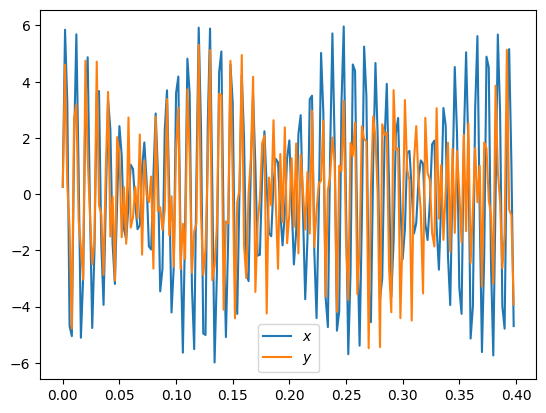
\includegraphics[width=.6\textwidth]{png/xy_graph.png}
	\caption{График сигналов $x,\,y$.}
	\label{xy_graph}
\end{figure}

{
	\foreach \i in {5,...,7}{
		\begin{center}
			\includegraphics[width=.6\linewidth]{png/csd_\i.png}
			\captionof{figure}{Спектральная плотность мощности}
			\label{csd_graph2_\i}
		\end{center}
	}
}

\section{Выводы}

В данной работе была рассмотрена методика анализа временных рядов. Был рассмотрен и реализован подход к выделению аномальных наблюдений с помощью эллипса рассеяния. Сформировали процедуры определения стационарности временного ряда, за счёт анализа блочных оценок математического ожидания $\hat{m}_y$ и дисперсии $\hat{\sigma}^2_y$. Для рассмотренных временных рядов критерий серий не определил наличия нестационарности. На наличие тренда в сигнале $y_3 (t)$ указывал только график автокорреляционной функции.

Были реализованы функции нахождения корреляционной функции $\hat{R}_{xy}(\tau)$ и собственной спектральной плотности мощности $\hat{S}_{xx}(f)$. Для их проверки построили и проанализировали оценки этих характеристик на типовых сигналах. Также сравнили использование различных оконных функций при построении периодограммных оценок.


